\documentclass[10pt]{article}
\usepackage[T1]{fontenc}
\usepackage[utf8]{inputenc}
\usepackage[margin=0.75in]{geometry}
\usepackage{booktabs}
\usepackage{tabularx}
\usepackage{array}
\usepackage{float}
\usepackage{xcolor}
\usepackage{graphicx}
\usepackage{hyperref}

\newcolumntype{Y}{>{\raggedright\arraybackslash}X}
\newcolumntype{L}[1]{>{\raggedright\arraybackslash}p{#1}}
\newcommand{\cmdpath}[1]{{\scriptsize\path{#1}}}

\title{SPPA-MVFit Submission Supplement: Protocol, Sealed Results, and Claim Boundaries}
\author{}
\date{}

\begin{document}
\maketitle
\vspace{-2.2em}

\section*{Purpose}

This short supplement is the formal companion for the SPPA-MVFit paper. The
longer historical technical diary is \textbf{not} submitted. This document
records the sealed confirmatory protocol path, key hashes, and claim boundaries.
Primary scientific tables appear in the main paper.

\section*{Primary endpoint (held-out)}

\begin{itemize}
\item Estimand: clean 64-cubed voxel IoU of \texttt{sppa\_mvfit} minus
\texttt{generic\_mvfit}.
\item Units: 240 source actors (12 family\(\times\)stratum cells, equal weight).
\item Decision: stratified bootstrap 95\% CI lower bound \(> +0.030\).
\item Result: mean \(\Delta=0.190\), CI \([0.181,0.199]\), \textbf{H1 PASS}.
\item Strata: CSG-ID \(0.209\), implicit-OOD \(0.172\) (both positive).
\item Provenance: \texttt{synthetic\_geometry} only.
\end{itemize}

\section*{Reproduction commands}

Run from the git repository root that contains the
\texttt{paper\_semantic\_proxy\_3d} junction (or paper directory). Do not
re-optimize the sealed held-out methods after inspection.

\begin{table}[H]
\centering
\footnotesize
\setlength{\tabcolsep}{3pt}
\renewcommand{\arraystretch}{1.08}
\caption{Minimal checks for the submitted primary claim.}
\begin{tabularx}{\linewidth}{@{}L{0.42\linewidth}Y L{0.16\linewidth}@{}}
\toprule
Command & Purpose & Expected \\
\midrule
\cmdpath{python -m pytest paper_semantic_proxy_3d/reproducibility/sppa_mvfit/tests/test_contract.py} &
Shared builder, budget, no cross-imports, split balance. &
7 passed \\
\cmdpath{python paper_semantic_proxy_3d/reproducibility/sppa_mvfit/benchmark/verify_package.py --development} &
Development package integrity. &
PASS \\
\cmdpath{python paper_semantic_proxy_3d/reproducibility/sppa_mvfit/benchmark/export_paper_tables.py} &
Regenerate main-paper tables from sealed \texttt{raw\_metrics.csv}. &
writes \texttt{.tex} \\
\cmdpath{python paper_semantic_proxy_3d/tools/reproduce_sppa_mvfit_paper.py --strict} &
Hash/gate checks for the submission snapshot. &
0 blockers \\
\bottomrule
\end{tabularx}
\end{table}

Held-out generation/evaluation commands exist in
\texttt{reproducibility/sppa\_mvfit/README.md} and require the protocol PASS
record, pretest freeze, and NIST-bound seed manifest. Re-running method
optimization for a better score is forbidden by protocol.

\section*{Selected sealed hashes}

\begin{itemize}
\footnotesize
\item Pretest freeze SHA-256:
\texttt{8E2ADBF32F299B24CD2A5AB87C74D142E707696F79D18DF0C3332209C3B46CA3}
\item Protocol PASS SHA-256:
\texttt{2348946BDDB04B8E5CA7D2C845C5F5C45F1AE06F8907E99218ED5E9A379FA74F}
\item Sealed predictions binary SHA-256:
\texttt{F870C57D9CC6FF4868EFB25FD2926FA7D19858EAF8CD0E9781F38990D7D145FD}
\item Raw metrics SHA-256:
\texttt{57A82D234F55013D76BEF2E36CF2B3F7C5617DD4FA6EF811C2A8447A04C0AD63}
\end{itemize}

\section*{Claim boundaries}

Supported: family-conditioned occupancy gain under synthetic calibrated
silhouettes; shared generator; optional runtime contract evidence.

Not supported: measured flight, real-UAV 3D GT accuracy, operator benefit,
universal open-set geometry, or neural image-to-3D SOTA ranking.

Real-image figures in the main paper and in this supplement remain qualitative
probes without 3D ground truth and use declared replay assumptions where
telemetry is shown.

\section*{Supplementary figures}
\renewcommand{\thefigure}{S\arabic{figure}}
\setcounter{figure}{0}

The two audit artifacts below are referenced from the main paper as
Supplementary Figures~S1 and~S2. They duplicate no main-paper figure: S1
provides the zoomed detector-evidence detail that the compressed comparison
grid cannot show, and S2 provides the multi-view renders behind the visual part
evidence audit table.

\begin{figure}[H]
\centering
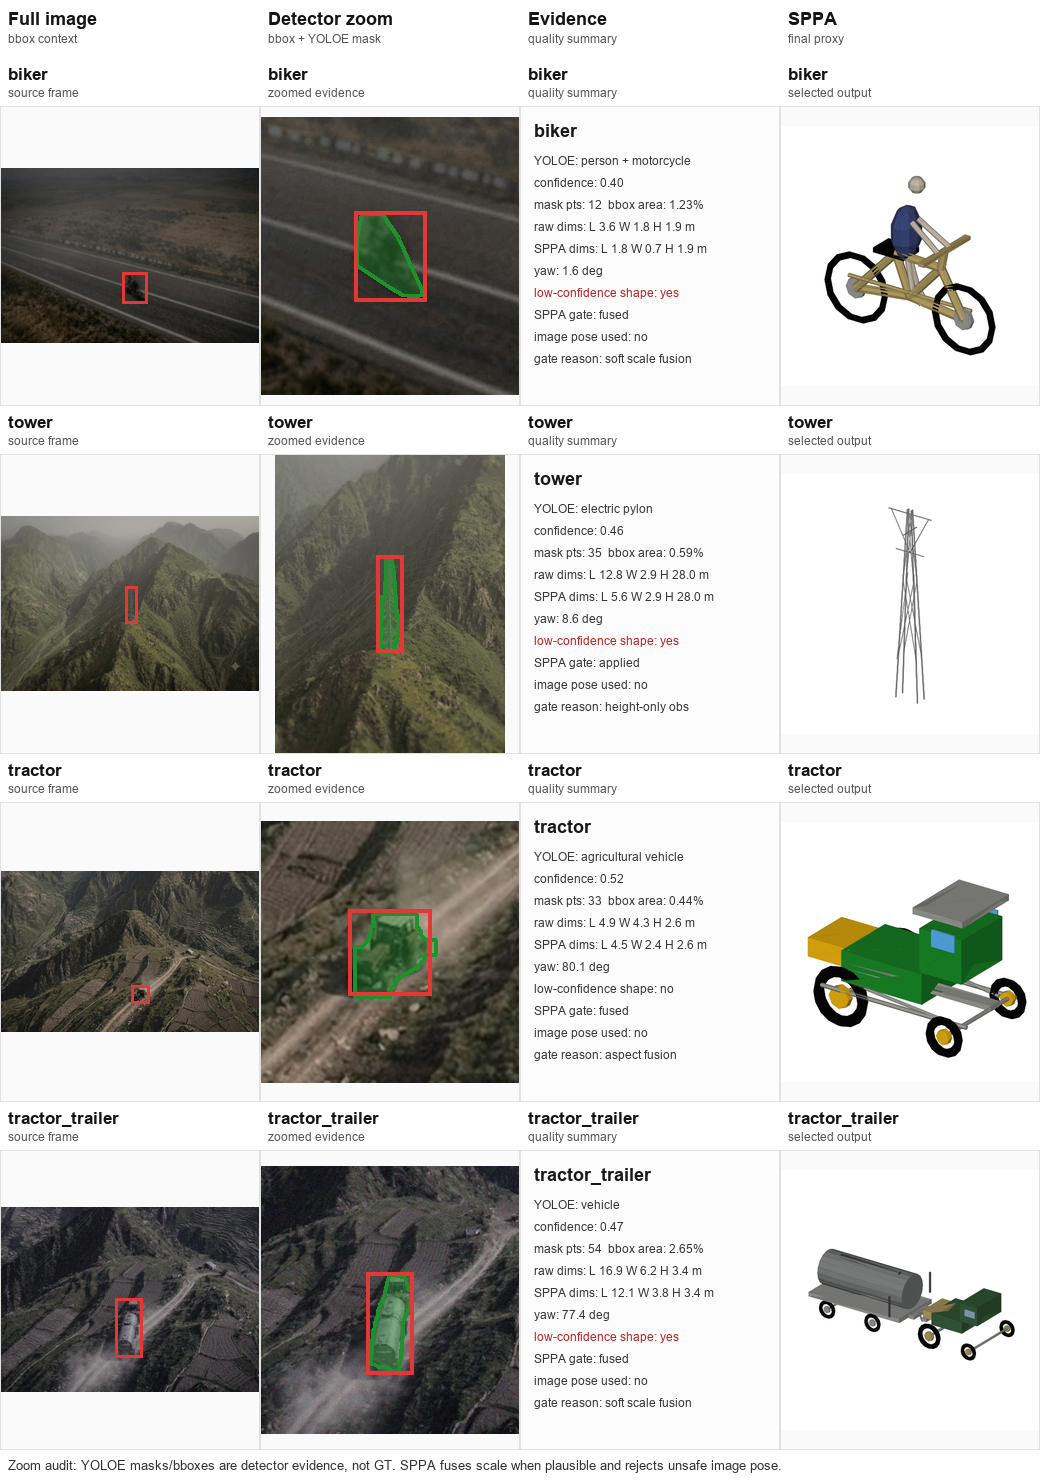
\includegraphics[width=\linewidth,height=0.75\textheight,keepaspectratio]{figures/sppa_real_detection_zoom_audit.png}
\caption{Zoomed real-input audit for the four user-supplied probes. Red boxes
and green masks are YOLOE detector evidence. The evidence panel reports
confidence, mask size, bbox area, inferred replay dimensions, yaw, and the
SPPA low-confidence shape flag. The zoom panel shows the final selected proxy;
the separate input-mode ablation reports text-only, detector+metric, and
detector+metric+visual variants. The evidence panel reports raw detector dimensions and
the final SPPA dimensions, showing that the tractor's nearly square footprint is
not copied but corrected through the vehicle aspect prior, while low-confidence
image pose is not used. SPPA recipes include
explicit connector primitives for semantically attached parts, such as bicycle
frame tubes, tower braces, tractor axles, and tractor-trailer hitch/axle
connectors. The full frames in the first column are also the real-image replay
evidence: red boxes are the selected YOLOE or composite detector bboxes and
green polygons are the native YOLOE/Ultralytics mask contours used by the
observation bridge, which remain detector evidence rather than ground-truth
masks.}
\end{figure}

\begin{figure}[H]
\centering
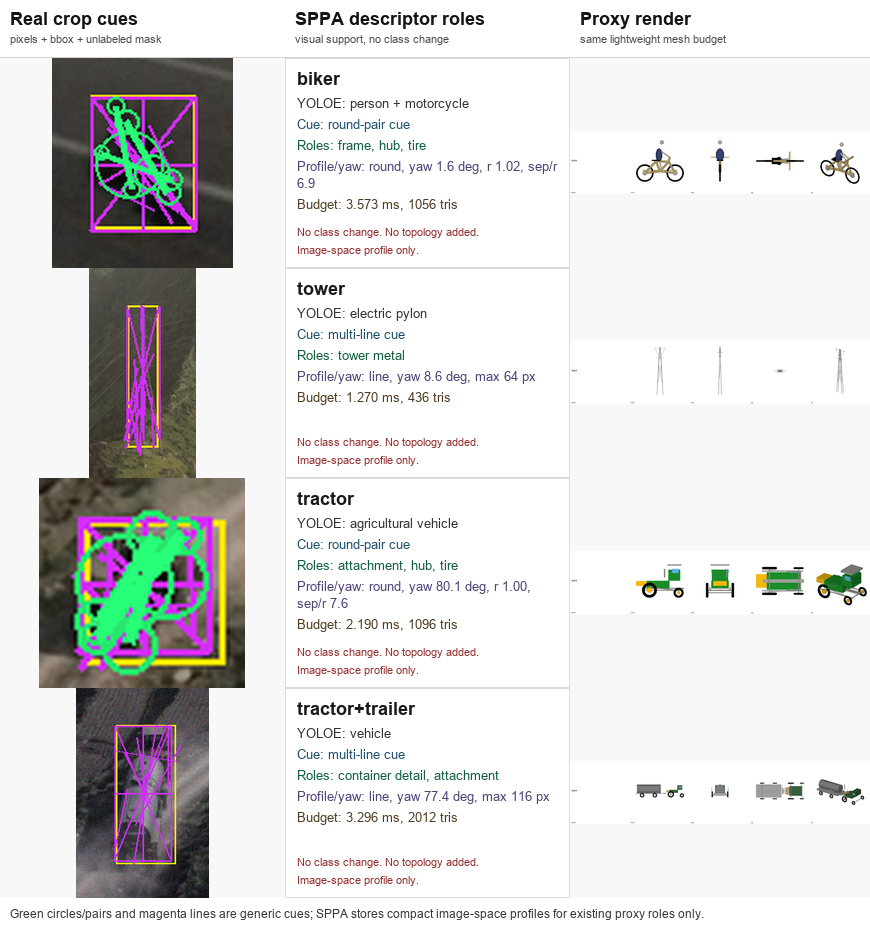
\includegraphics[width=\linewidth]{figures/sppa_visual_part_evidence_grid.png}
\caption{Visual part evidence bridge on the four real probes. Green
circles/pairs and magenta lines are generic image-space cues from pixels,
detector boxes, and unlabeled mask geometry. SPPA maps those cues only onto
descriptor roles already present in the selected proxy and records a compact
image-space geometry profile; when the visual--metric gate is non-divergent, the
selected yaw is the declared-replay axial footprint yaw. The semantic class and
mesh topology are unchanged.}
\end{figure}

\end{document}
